\documentclass{article}
\usepackage{amsmath}
\usepackage{hyperref}
\usepackage{tikz}
\begin{document}

\title{Electro Magnetic Interference and HF Radio Receivers}
\maketitle

\section{Introduction}
 
Throughout the 20th century HF radio receiver technology evolved with the aim of detecting distant, narrow band signals.  Radio noise sets the limits of detection \cite{itu372}, and was assumed to be from natural sources or the receiver itself. However in the early 21st century, from lower HF right up to UHF noise from human activity now dominates the detection problem.  We are no longer seeking to maximise signal-to-noise ratio (SNR), but signal to EMI ratio (SER).

We are slowly losing the ability to use analog SSB in urban areas.  Many Hams report S9 noise levels, $9 \times 6 = 54$ dB Hams higher than a quiet S0 country station.  Consequently, digital modes that can operate operate at low SERs are becoming popular.  Digital modes are in an arms race with EMI.

Our target radio signals are from distant sources, weak, narrow band, and evolve slowly in time. Human generated radio noise tends to be very strong, wideband, with a time domain envelope that evolves quickly in time.  It is often radiated from nearby sources, such as power lines lines and house wiring a few 10s of meters from our antenna.  It has significant structure, so can be interpreted as an interfering signal, rather than random noise.

Modern radios are very good at rejecting strong unwanted narrowband signals, using frequency selectivity and good strong signal performance.  This report explores ways we can reject human made noise in the lower HF bands.

\section{Radio Noise Signals from Human Activity}

Table \ref{table:human_noise} is a summary of human generated noise sources.  The values are approximate and based on the authors experience - your mileage may vary!  This categorisation gives us some insight that can be used to classify signals, consider their impact, and possible attacks.

The Time and Frequency columns describes the distribution of energy in time and frequency, for example power line arcing can cause clicks in our radio similar to atmospheric lightning.  The noise signal consists of short, powerful time domain pulses that are randomly distributed in time, resulting in wideband energy uniformly distributed in frequency. It may be identified and removed via noise blanking techniques.

In contrast DSL signals radiated from leaky phone lines looks like noise in the time domain and frequency domain, making it particularity hard to identify and remove.  It is very similar to AWGN from natural noise sources.

Bandwidth relates the rate $R$ of the noise pulses to the bandwidth $B$ of a typical SSB HF receiver (around 3000 Hz).  When $R<<B$, we tend to hear individual noise pulses, and separate pulses can be observed in a time domain plot of the receiver output waveform.  When $R>B$, we hear just a bandpass segment of the EMI signal, for example a tone from a PWM harmonic, or some modulated wideband noise.

Our narrow band receiver smooths the time domain envelope. As $R$ relative to $B$ increase, our receiver converts a series of short time domain pulses (such as a PWM waveform) into a longer pulses with a smooth time domain envelope (AWGN noise), making the EMI signal harder to identify and remove.

If we position our receiver some distance from many urban noise signals (for example the middle of an urban park), we get the sum of many signals added together, which converges to AWGN noise.  The level reduces with distance, so an effective attack is decamping to a country location, and operating a portable station for the day.

For an EMI signal to be transmitted, we need a source of AC current and an antenna. Domestic electricity lines appear to operate in a mode part way between transmission line and antenna.  RF does seem to propagate along them quite well, they then radiate quiet strong signals to nearby homes.  Likewise, DSL signals on ancient phone lines are poor transmission lines and and reasonably effective antennas, radiating significant local EMI. A home with buried electricity lines and fibre or wireless supplying Internet is desirable.

\begin{table}[h]
\centering
\begin{tabular}{l l l l l l}
 \hline
 Name & Rate & Time & Frequency & Antenna & BW \\
 \hline
 Power Line & 1 Hz & random pulse & uniform & power lines & $R < B$ \\
 Downlights & 50-60 Hz & pulse train & harmonics & house wiring & $R < B$ \\
 SMPS & 10-300 kHz & pulse train & harmonics & house wiring & $R > B$ \\
 DSL & 1-12 MHz & AWGN & AWGN & phone lines & $R > B$ \\
 Urban Sum & lower HF & AWGN & AWGN & power lines & $R > B$ \\
 \hline
\end{tabular}
\caption{Summary of Radio signals from Human Activity}
\label{table:human_noise}
\end{table}

The modulation used in our desired target signals is a factor.  Digital modes can operate at lower SNRs than analog SSB.  Digital modes can also use Forward Error Correction (FEC), for example we can correct a bit error caused by a noise impulse wiping out one bit.  Digital modulation also has a threshold effect - once the interference is a few dB lower than the wanted signals, it's impact on bit errors is small. FM, FSK \& PSK are more robust to impulsive noise than amplitude modulated modes like SSB.

\section{EMI from Pulse Trains}
\label{pwm}

\subsection{Pulse Width Modulation}
\label{smps}

The PWM switch mode power supply is a ubiquitous source of interference.  Consider the Fourier Series of an ideal pulse train \cite{wikipedia_pulse}:
\begin{equation} \label{eq_pwm}
\begin{split}
x(t) &= Ad+\frac{2A}{\pi} \sum_{n=1}^{\infty} \frac{sin(\pi n d)}{n}cos(n \omega t) \\
     &= Ad+\frac{2A}{\pi} \sum_{n=1}^{\infty} \frac{x(t)}{n} cos(n \omega t)
\end{split}
\end{equation}
where $0<d<1$ is the duty cycle and $\omega=2 \pi R$ the fundamental frequency.  The Fourier series is a sequence of harmonics $cos(n \omega t)$, with the amplitude of each harmonic set by the $x(t)/n$ term. A typical value for $R$ is a few kHz to several hundred kHz. For example with R = 70kHz and $n=101$ we will have a harmonic at 7.1 MHz. The $1/n$ factor means the power of each harmonic falls off slowly with frequency, e.g. the $n=100$ harmonic will be just $10log_{10}(1/100)=-20$ dB down compared to the fundamental ($n=1$) power, and the $n=101$ harmonic almost the same power at $10log_{10}(1/101)=-20.043$ dB down.

If the duty cycle $d$ is constant, then each harmonic is an unmodulated sine wave of constant amplitude. In practice $d$ is time varying, as the duty cycle is continuously adjusted by the power supply.  This leads to modulation of each harmonic $x(t)$, spreading the power to frequencies either side of the harmonic centre $n \omega$.

Let $d$ have a constant and time varying component:
\begin{equation}
d=d_c+ad(t)
\end{equation}
where $d(t)$, $|d(t)| \le 1$ is a PWM modulation function and $a$ is the peak amplitude of the modulation (ie the peak jitter of the PWM signal). For the $n$-th harmonic:
\begin{equation} \label{eq:pwm_n}
\begin{split}
x_n(t) &= sin(\pi n d) \\
       &= sin(\pi n (d_c+ad(t)) \\
       &= sin(\pi n d_c + \pi n a d(t)) \\
       &= sin(\pi n d_c + h d(t))  \\
     h &= \pi n a
\end{split}
\end{equation}
It can be seen that $h$ is strong function of $a$, as small changes are multiplied by $n \pi$. For example for $n=100, a=0.01, h = \pi$.  Thus with just 1\% jitter of the PWM signal, a cycle of $d(t)$ would modulate over the entire $\pm \pi$ range of the $sin()$ function.

We would like to estimate the spectrum of $x(t)$. First we consider small $h << 1$:
\begin{equation} \label{eq:small_h}
\begin{split}
x_n(t) &= sin(\pi n d_c)cos(hd(t)) + cos(\pi n d_c)sin(hd(t)) \\
       &\approx sin(\pi n d_c)(1 - (hd(t))^2/2) + cos(\pi n d_c)hd(t) \\
       &\approx sin(\pi n d_c) + hcos(\pi n d_c)d(t)
\end{split}
\end{equation}
The LHS is a constant term related to the mean duty cycle of the PWM signal, the RHS is linear modulation term, i.e. a small linear modulation about a mean set point.  When multiplied by the $n$-th harmonic $cos(n \omega t)$ in (\ref{eq_pwm}):
\begin{equation}
\begin{split}
x_n(t)cos(n \omega t) &= \left[ sin(\pi n d_c) + hcos(\pi n d_c)d(t) \right] cos(n \omega t) \\
                      &= sin(\pi n d_c)cos(n \omega t)) + hcos(\pi n d_c)d(t)cos(n \omega t) \\
                      &= c_1 cos(n \omega t)) + c_2 d(t)cos(n \omega t) \\
                   c_1 &= sin(\pi n d_c) \\
                   c_2 &= hcos(\pi n d_c)
\end{split}
\end{equation}
By examining the different frequency terms we can estimate the spectrum of the PWM signal near the n-th harmonic. Note $c_1$ and $c_2$ are constants that do not affect the number of different frequency terms. The LHS of (\ref{eq:small_h}) is a constant carrier term at the harmonic centre. The product of $d(t)cos(n \omega t))$ will produce images of the spectra of d(t) either side of $n \omega$. This is Amplitude Modulation (AM).  For example if $d(t)$ is a random variable with maximum frequency $\omega_m$ radians, we would see a uniform noise spectrum over the interval $n \omega \pm \omega_m$, with a central "carrier" spectral line at $n \omega$. If $\omega_m > \omega/2$, the entire region between each harmonic will have additive white noise generated from the PWM signal.

For larger $h$, Equation \ref{eq:pwm_n} can be interpreted as Phase Modulation (PM) \cite{wikipedia_phase} of a zero frequency carrier. Assuming a random $d(t)$, the resulting spectra of $x(t)$ can be approximated using Carsons Rule, as having 98\% of it's power contained within $B_c=2(h+1)f_m$ Hz, where $f_m$ is the maximum frequency component of $d(t)$. When multiplied by the $cos(n \omega t)$ term, the PM signal will spread the power of the carrier over range of adjacent frequencies, replacing the PWM carrier in the small $h$ case with a band of white noise.

For example, let $a=0.02$ (a few percent jitter of the PWM duty cycle) and the bandwidth of the PWM control loop be $f_m=3$ kHz. At $n=100$ we have $h=\pi n a = 2\pi$, which implies a random deviation of $\pm 2\pi$ (two cycles of $sin()$), and an $x(t)$ bandwidth of $B_c=2(2 \pi+1)f_m = (4\pi+2)f_m = 43$ kHz.

\subsection{Discussion}

\begin{enumerate}
\item Given $h$ increases with $n$, we can expect to see AM type modulation either side of central harmonics lines at lower frequencies.  At intermediate frequencies a raised noise floor will be observed between harmonics.  As the frequency increases further the power of the harmonics lines will reduce and gradually be replaced by broadband noise.
\item With the common scenario of a receiver of bandwidth $B<R$, we would encounter sine wave "carriers" every R kHz as we tune.  Tuning between carriers would expect to hear a bandpass version of $d(t)$, this may or may not be white.  If not white, it may have structure we can exploit. It may also be periodic, of quasi-stationary.
\item With a large number of PWM sources, the central limit theorem suggests the sum will converge to AWGN noise with very little structure in time or frequency.  This may the case with signals radiated from electricity power lines that are coupled to thousands of switch mode power supplies in a city.
\item In the local case, it is possible that switch mode PWM or impulse noise may dominate a particular receiving station.
\end{enumerate}

\subsection{Periodic Impulse Noise}

Section \ref{smps} explored the spectra of PWM power supplies which typically have a pulse rate $R$ greater than the receiver bandwidth $B$ (e.g. $B=3000$Hz for SSB signals on HF radio). A low frequency pulse train (such as ignition or $R=50 \ldots 60$ Hz impulses from domestic lighting) can also be interpreted as a pulse train with small duty cycle $d$, and $R<<B$.  In this case there will be a number of harmonics inside our receiver passband.  Consider (\ref{eq_pwm}), band pass filtered such that only harmonics $n_1 \ldots n_2$ remain:
\begin{equation}
\begin{split}
x(t) &= Ad+Ad\sum_{n=1}^{\infty} sinc(\pi n d) cos(n \omega t) \\
BPF \left[ x(t) \right] &= Ad\sum_{n=n_1}^{n=n_2} sinc(\pi n d) cos(n \omega t)
\end{split}
\end{equation}
Shifting down to baseband, and making the substitution $k=n-n_1$:
\begin{equation}
\begin{split}
BPF \left[ x(t) \right] cos(n_1 \omega t) &= \frac{Ad}{2} \sum_{k=0}^{n=n_2-n_1} sinc(\pi (k+n_1) d) cos(k \omega t) \\
&+ \frac{Ad}{2} \sum_{k=0}^{n=n_2-n_1} sinc(\pi (k+n_1) d) cos((k+n_1) \omega t) \\
&= b(t) + c(t)
\end{split}
\end{equation}
By applying a low pass filter we are left with the baseband term $b(t)$:
\begin{equation}
\begin{split}
b(t) &= \frac{Ad}{2} \sum_{k=0}^{n=n_2-n_1} sinc(\pi (k+n_1) d) cos(k \omega t) \\
     &= \frac{Ad}{2} + \frac{Ad}{2} \sum_{k=1}^{n=n_2-n_1} sinc(\pi n_1 d + \pi k d) cos(k \omega t)
\end{split}
\end{equation}
This expression is similar to the Fourier Series for a pulse train (\ref{eq_pwm}), but limited to $n_2-n_1$ harmonics by the bandwidth $B$ of the receiver.  The baseband signal $b(t)$ can therefore be interpreted as a periodic signal with the same period $\omega$ as the wideband periodic impulse noise $x(t)$.  The shape of the pulse train will be a modified version of the $x(t)$, as we are using a band pass set of $sinc()$ coefficients.  Given $d$ is likely to be small (e.g a $10 \mu$s pulse every 20ms), and $n_2-n_1 << n_1$, the coefficients are likely to be similar in amplitude across $n_1 \ldots n_2$, producing a high peak to average power (low duty cycle) ratio pulse train.

Given $d$ is small, and there is still significant power at high harmonic numbers, $A$ must be very large for these impulse noise sources.

\subsection{Attacks}

\begin{enumerate}
\item Estimation and subtraction of the signals. Key take away is mirror of $d(t)$ about harmonic centre. Estimation of signal from one sideband to cancel other, or from AM demodulation (envelope). This will be problematic when it's spread so far that we get energy from $n+1$, $n-1$ near harmonic $n$.  However in that case it may not be as annoying/strong.

\item Estimation of signal from adjacent harmonics.  Can we find $x_n(t)$ from $x_{n-1}(t)$?  $\omega$ and $n$ can be estimated from the spectrum.  A direct form solution is unlikely however the equations are differentiable so an iterative solution could be found.

\item Dual channel coherent removal.

\item Noise blanking in the time domain.  This may be challenging with $R>100$ kHz, as the period becomes $< 10\mu$s, implying the need for a wide bandwidth and sample rate $>>100$ kHz in order to resolve individual noise pulses in the time domain.

\item Training of time domain pulses, correlation and removal.
\end{enumerate}

\section{Noise Blanker}

Consider a signal $x(t)$ consisting of a wanted sinusoidal signal and an unwanted impulse train that repeats every $1/R$ seconds.
\begin{equation}
x(t) = a_1 e^{j \omega_1 t} + a_{imp}\sum_{n=-\infty}^{\infty}\delta(t-n/R)
\end{equation}
To remove the impulse, a blanking pulse train $b(t)$ is applied.  Each pulse is $T$ seconds wide:
\begin{equation}
\begin{split}
b(t) &= 1 - p(t) \\
p(t) &= \sum_{n=-\infty}^{\infty}rect(t-n) \\
rect(t) &= 
	\begin{cases}
      1, & |t| <= T/2 \\
      0, & otherwise \\
	\end{cases} \\
\sum_{n=-\infty}^{\infty}\delta(t-n/R) b(t) &= 0
\end{split}
\end{equation} 

\begin{figure}[h]
\caption{Blanking Pulse $b(t)$ }
\vspace{5mm}
\label{fig:rect_time}
\centering
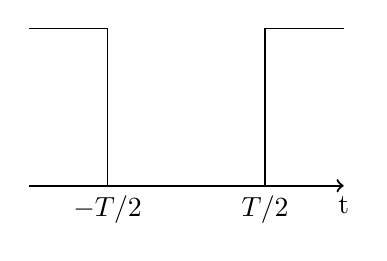
\begin{tikzpicture}
\draw[thick,->] (1,0) -- (5,0) node [below]{t};
\draw (1,2) -- (2,2) -- (2,0) node [below]{$-T/2$} -- (4,0) node [below]{$T/2$} -- (4,2) -- (5,2);
\end{tikzpicture}
\end{figure}

The pulse train $p(t)$ can be expressed as Fourier Series (\ref{eq_pwm})
\begin{equation}
\begin{split}
p(t) &= d+\frac{2}{\pi} \sum_{n=1}^{\infty} \frac{sin(\pi n d)}{n}cos(n \alpha t) \\
     &= d + d \sum_{n=1}^{\infty} sinc(\pi n d) \left[ e^{-j\alpha n t} + e^{j \alpha n t} \right] \\
     &= d + d h(t) \\
h(t) &= \sum_{n=1}^{\infty} sinc(\pi n d) \left[ e^{-j\alpha n t} + e^{j \alpha n t} \right]  
\end{split}
\end{equation}
where $\alpha=2 \pi R$ is the angular frequency of the pulse train, $d=TR$ is the duty cycle, and $h(t)$ is the RHS term containing the harmonics.  The Fourier Transform of $h(t)$ is:
\begin{equation}
\begin{split}
H(w) &= \int_{-\infty}^{\infty}h(t)e^{-j \omega t}dt \\
     &= \int_{-\infty}^{\infty} \sum_{n=1}^{\infty} sinc(\pi n d) e^{-j\alpha n t}e^{-j \omega t}dt \\
     &+ \int_{-\infty}^{\infty} \sum_{n=1}^{\infty} sinc(\pi n d) e^{j\alpha n t}e^{-j \omega t}dt \\
     &= \sum_{n=1}^{\infty} sinc(\pi n d) \left[ \delta(\omega + \alpha n) + \delta(\omega - \alpha n) \right]
\end{split}
\end{equation}
The frequency shifted Fourier transform of $h(t)e^{j \omega_1 t}$ is
\begin{equation}
\begin{split}
\int_{-\infty}^{\infty} h(t)e^{j \omega_1 t} e^{-j \omega t}dt &= H(\omega-\omega_1) \\
  &= \sum_{n=1}^{\infty} sinc(\pi n d) \left[ \delta(\omega + \alpha n - \omega_1) + \delta(\omega - \alpha n - \omega_1) \right]
\end{split}
\end{equation}

Consider the output of the noise blanker:

\begin{equation}
\begin{split}
y(t) &= x(t)b(t) \\
     &= a_1 e^{j \omega_1 t} - a_1 e^{j \omega_1 t}p(t) \\
     &= a_1 e^{j \omega_1 t} - a_1 e^{j \omega_1 t}(d + dh(t)) \\    
     &= a_1 (1-d) e^{j \omega_1 t} - a_1 d h(t) e^{j \omega_1 t} \\    
Y(w) &= a_1 (1-d) \delta(\omega - \omega_1) - a_1 d H(\omega-\omega_1) \\
     &= a_1 (1-d) \delta(\omega - \omega_1) \\
     &- a_1 d \sum_{n=1}^{\infty} sinc(\pi n d) \left[ \delta(\omega + \alpha n - \omega_1) + \delta(\omega - \alpha n - \omega_1) \right]
\end{split}
\end{equation} 

\begin{figure}[h]
\caption{Two examples of Noise Blanker output spectrum $|Y(f)|$.  The green lines show a typical SSB radio bandwidth of $B=3000$ Hz. Top is pulse rate $R<B$, bottom with $R>B$.  Note the harmonic level increasing with duty cycle $d=TR$, and how the harmonics fall outside of $B$ on the bottom plot. }
\label{fig:train_e_mean}
\begin{center}
\input blanker.tex
\end{center}
\end{figure}

\subsection{Discussion}

\begin{enumerate}
\item The wanted signal has been reduced to $(1-d)$, and harmonics $H(\omega)$ have been introduced either side.
\item The harmonics level are proportional to the duty cycle $d$.
\item If the harmonic levels approach $a_1$ they may cause interference.  However for PSK waveforms a margin of only a few dB beneath the wanted signal would be acceptable.  This suggests digital waveforms can benefit more from noise blanking than analog. 
\item A second, strong signal in the processing bandwidth could introduce interference if one of it's harmonic sidebands approaches $a_1$ at $\omega_1$.  This is the intermodulation effect of noise blankers.
\item The PWM analysis in Section \ref{pwm} showed that a small duty cycle/small jitter signal can cause broadband noise.  This suggests a narrow time domain blanking pulse $T<<1/R$ can remove that noise with acceptable impact on the wanted signal. 
\item With noise/blanker pulse rates $R>B$, the harmonics are separated by $R$, so blanker harmonics are likely to be outside of our target pass band $B$.  However intermodulation effects are larger, so strong signals further away could be aliased into our passband. 
\item So far a rectangular blanking pulse has been assumed. A smoother function for $p(t)$ is likely to reduce the level of $H(\omega)$. 
\end{enumerate}

\section{Experimental Results}

In May 2023 a series some experimental work was conducted at the authors suburban home.  The goal was to gain experience in measuring EMI and attempt to fit the experimental results to the theoretical framework above.

The home is located Adelaide (population 1 million), South Australia and is on a suburban square corner block of 500 m^2.  Overhead power lines are on two sides, and the suburb is served by VDSL Internet using 70 year old twisted pair.  

The station antenna is an inverted V fan dipole with 40m and 20m elements, suspended over the house, the mast and feed point is 9m above ground. It is coupled to 50 ohm coax using a balun. Subjectively, SSB stations on the 40m band are hard to hear and unpleasant to listen to, and 20m varies between low noise levels and completely unusable (time varying).

TODO figure, Google map?

TODO table of noise levels, levels, frequency, classification

If we want to manage noise, we first need to measure it.
use of S-meter, spec-an, waterfall displays, scope

establish baseline goal against these measurements

Dual antenna experiments, Afredri, had to wind gain dowsn due to strong local broadcast signals, increased noise figure.

\subsection{Discussion and Conclusion}

The dominant EMI on both bands is AWGN, which is the sum of many urban EMI signals. We cannot attack this with blanking, as it has no time domain pulse structure.  This leaves diversity, which requires the received signal on antenna 1 to be related to the signal received on antenna 2 by a single complex coefficient:
\begin{equation}
r_1(t)=cr_2(t)
\end{equation}
This implies the target EMI signal must be above the receiver noise floor in both channels (TODO extend expression for this, maybe include uncorrelated near field).

In diversity systems the two antennas are placed some fraction of a wavelength apart. Near field intensity is a strong function of distances of less than one wavelength, so the two antennas are likely to have very different responses to near field EMI. For example at a spacing of $\lambda/4$ a near field signal coupled to one antenna may be undetectable in the other antenna. This implies the EMI fields must be fully resolved far field signals for the diversity attack to work.  Alternatively antennas with very small separation should be used such that near field signals are detected at adequate levels in both antennas.

Near field signals can be induced in antenna systems by common mode injection into feed lines and antenna conductors. We should take steps to reduce any near field signals by routing feed lines and antennas away from near field sources such as house and street wiring, and using balanced antenna systems.

However physical distancing is problematic on small urban blocks, where any antenna is likely to be less than one wavelength from conductors radiating EMI.

Antenna topologies may help reduce near field detection.  For example the conductors of physically small, non resonant loops and dipoles can be placed further away from near field sources compared to a full length dipole that must extend across the entire side of an urban block.

Height rather than x-y separation
Preamplifier located at feedpoint, so increase teh ratio of rx signal to common mode feedline (maybe, depends how it gets in I guess).
common mode chokes

Need for objective testing

Beam antenna, as AWGN noise field is likely not a point source, but the sum of many signals received from all directions, so N the same, S will increase for point source wanted signal


TODO: figure

The loop in/on ground topilogy has been proposed.  While this would not naturally reduce 

discussion of antenna topologies (refs to log in ground, small loops), common mode feedline.  Small non resonant loops that don't couple (ref)

next steps, core aim of testing theory that AWGN "urban sum" can be supressed using coherent methods

identical antennas, loops to ensure good balance, small to enable placing away from near field.
measure noise figure
BCI filter
A way to measure SNR, e.g. car Tx, log signal as I drive around, on two channels, try loop v diople, control for azimuth
 
model, EMI as sum of several signals


\bibliographystyle{plain}
\bibliography{emi_refs}
\end{document}
